\section{Galaxy collision}
\subsection{P3M method}
\begin{figure}[htp]
    \centering
    \begin{subfigure}[b]{0.45\textwidth}
        \centering
        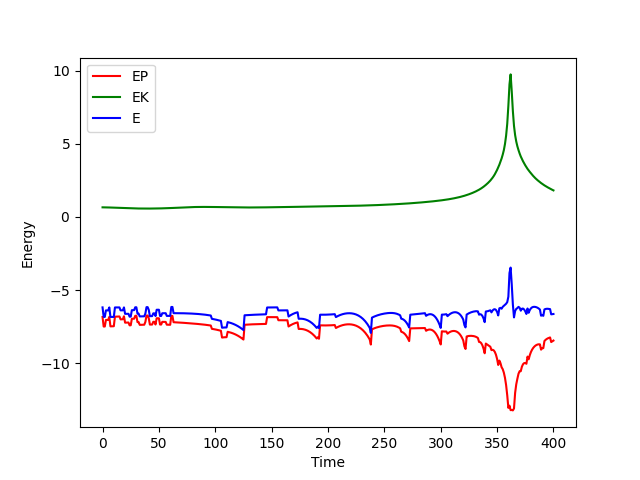
\includegraphics[width=\textwidth]{chapters/results/img/p3m-collision/energy.png}
        \caption{Energy}
        \label{fig:physical-quantities-p3m-collision-sub1}
    \end{subfigure}
    \hfill
    \begin{subfigure}[b]{0.45\textwidth}
        \centering
        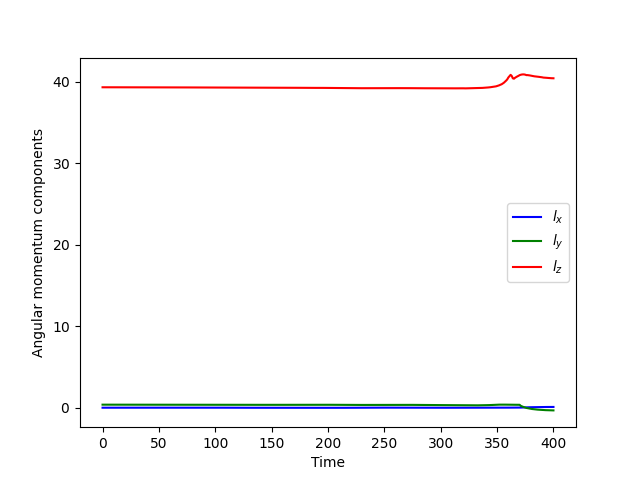
\includegraphics[width=\textwidth]{chapters/results/img/p3m-collision/angular-momentum.png}
        \caption{Angular momentum}
        \label{fig:physical-quantities-p3m-collision-sub2}
    \end{subfigure}

    \vspace{0.2cm}

    \begin{subfigure}[b]{0.45\textwidth}
        \centering
        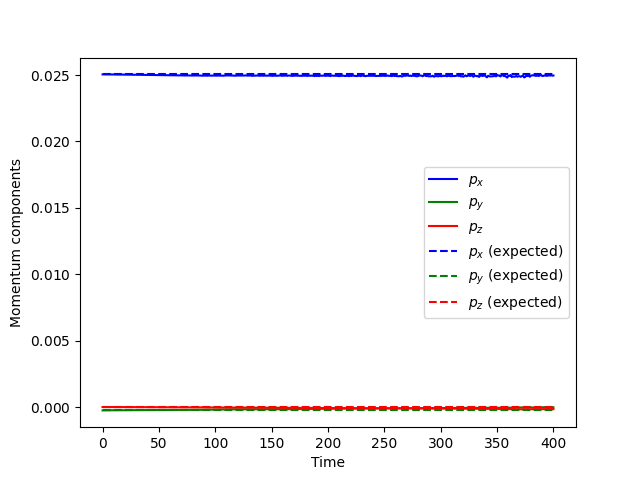
\includegraphics[width=\textwidth]{chapters/results/img/p3m-collision/momentum.png}
        \caption{Momentum; broken lines represent the expected momentum following \autoref{eq:expected-momentum-change}}
        \label{fig:physical-quantities-p3m-collision-sub3}
    \end{subfigure}

    \caption{Fundamental physical quantities describing the system over time in the Barnes-Hut algorithm.
        Time is in Myr and the quantities are expressed in units consistent with \autoref{tab:galaxy-parameters}}
    \label{fig:physical-quantities-p3m-collision}
\end{figure}